\begin{problem}
  Throughout these last two sections, we have tacitly assumed there exists a unique
  solution. That is not always the case. Consider the problem
  \[
    y'' + y = 0 \quad y(0) = y(\pi) = 0.
  \]

  There are infinitely many solutions, all of the form: $y = C\sin(x)$, where $C$
  is an arbitrary constant. Nevertheless, use the finite-element method to solve
  this problem. Take larger and larger values of $n$. Recall the theory of
  eigenvalues for matrices
\end{problem}

\begin{proof}
  We wish to find an approximation $y_n(x)$ to the exact solution $y = C\sin(x)$
  using the finite-element method employing the hat basis outlined in problem 4.
  The approximation will have the form
  \begin{align*}
    y_n(x) = \sum_{j=1}^n a_j \phi_j(x).
  \end{align*}
  where
  \begin{align*}
    \phi_j(x) :=
    \begin{cases}
      \frac{x - h(j-1)}{h} & \text{if $(j-1)h \leq x \leq jh$} \\
      -\frac{x - h(j+1)}{h} & \text{if $jh \leq x \leq (j + 1)h$} \\
      0 & \text{otherwise} \\
    \end{cases}
  \end{align*}
  and $h = \pi / (n + 1)$.

  Following the methods outlined in problem 2, we want the approximation to
  satisfy the equations
  \begin{align*}
    \int_0^\pi (y_n'' + y_n)\phi_i(x)dx = 0 \quad \text{for $i = 1,\dots,n$}.
  \end{align*}

  In order to practically solve the system, we rewrite the differential
  equation in the form presented in \eqref{alternate_diffeq} by
  choosing $p(x) = 1$, $r(x) = f(x) = 0$, and $q(x) = 1$. Thus,
  the system becomes
  \[
    \int_0^\pi ((p(x)y_n')' + r(x)y_n)\phi_i(x) dx = 0 \quad \text{for $i=1,\dots,n$}.
  \]
  Making use of the fact that the basis functions are 0 on the boundary we see that
  \begin{align*}
    \int_0^\pi (p(x)y_n')'\phi_i(x) dx
    &= \phi_i(x)p(x)y_n'\rvert_0^\pi - \int_0^\pi p(x)y_n'\phi_i'(x) dx \\
    &= - \int_0^\pi p(x)y_n'\phi_i'(x) dx.
  \end{align*}
  With this and the definitions of the functions $p(x)$ and $r(x)$,
  the system of equations becomes
  \begin{align}\label{system_imp}
    \sum_{j=1}^n a_j \int_0^\pi -\phi_j'(x)\phi_i'(x) + \phi_j(x)\phi_i(x) dx = 0\quad \text{for $i=1,\dots,n$}.
  \end{align}

  Proceeding as we did in problem 4, we see that each of the entries $a_{ij}$
  of the coefficient matrix $A$
  has a special structure and that we need only calculate the diagonal and sub-diagonal.

  Thus, there are only two cases two consider, $i = j$ and $i = j + 1$.
  In the first case, we see that for any $i$,
  \begin{align*}
    a_{ii}
    &= \int_{(i-1)h}^{(i+1)h}-\phi_i'(x)^2 + \phi_i(x)^2 dx \\
    &= \int_{(i-1)h}^{ih} - \left(\frac{1}{h}\right)^2 + \left(\frac{(x - h(i-1))}{h}\right)^2 dx +
    \int_{ih}^{(i+1)h} - \left(-\frac{1}{h}\right)^2 + \left(-\frac{(x - h(i+1))}{h}\right)^2 dx \\
    &= - \frac{2}{h} + \frac{2h}{3}.
  \end{align*}
  In the second case, we similarly see that
  \begin{align*}
    a_{i(i-1)} &=
    \int_{0}^1 -\phi_{i}'(x)\phi_{i-1}'(x) + \phi_{i}(x)\phi_{i-1}(x) dx \\
    &= \int_{(i-1)h}^{ih} -\left(\frac{1}{h}\right)\left(-\frac{1}{h}\right) + \left(\frac{x - h(i-1)}{h}\right)\left(-\frac{(x - hi)}{h}\right)dx
    = \frac{1}{h} + \frac{h}{6}
  \end{align*}
  Therefore,
  \begin{align*}
    a_{ij} =
    \begin{cases}
      - \frac{2}{h} + \frac{2h}{3} & \text{if $i = j$} \\
      \frac{1}{h} + \frac{h}{6} & \text{if $|i - j| = 1$} \\
      0 & \text{otherwise}.
    \end{cases}
  \end{align*}
  Thus, our system is given by
  \begin{align*}
    \renewcommand\arraystretch{1.5}
    \begin{bmatrix}
      - \frac{2}{h} + \frac{2h}{3} & \frac{1}{h} + \frac{h}{6} & \hdots & 0 \\
      \frac{1}{h} + \frac{h}{6} & - \frac{2}{h} + \frac{2h}{3} & \hdots & 0 \\
      \vdots & \vdots & \ddots & \vdots  \\
      0 & 0 & \hdots & - \frac{2}{h} + \frac{2h}{3} \\
    \end{bmatrix}
    \begin{bmatrix}
      a_1 \\
      a_2 \\
      \vdots \\
      a_n
    \end{bmatrix}
    =
    \begin{bmatrix}
      0 \\
      0 \\
      \vdots \\
      0 \\
    \end{bmatrix}.
  \end{align*}
  The astute observer will note that the solution to this system is in fact the
  trivial solution. We therefore make the following transformation to the system
  \begin{align*}
    \renewcommand\arraystretch{1.5}
    \begin{bmatrix}
      \frac{2}{h} & -\frac{1}{h} & \hdots & 0 \\
      -\frac{1}{h} & \frac{2}{h} & \hdots & 0 \\
      \vdots & \vdots & \ddots & \vdots  \\
      0 & 0 & \hdots & \frac{2}{h} \\
    \end{bmatrix}
    \begin{bmatrix}
      a_1 \\
      a_2 \\
      \vdots \\
      a_n
    \end{bmatrix}
    &=
    \renewcommand\arraystretch{1.5}
    \begin{bmatrix}
      \frac{2h}{3} & \frac{h}{6} & \hdots & 0 \\
      \frac{h}{6} & \frac{2h}{3} & \hdots & 0 \\
      \vdots & \vdots & \ddots & \vdots  \\
      0 & 0 & \hdots & \frac{2h}{3} \\
    \end{bmatrix}
    \begin{bmatrix}
      a_1 \\
      a_2 \\
      \vdots \\
      a_n
    \end{bmatrix} \\
    A_1 x &= M x \\
  \end{align*}

  The problem then becomes finding the eigenvector solution to the generalized
  eigenvalue problem $A_1 x = \lambda M x$ associated to the eigenvalue $\lambda = 1$.
  Thus, the eigenvector $x$ satisfying the equation is the vector of coefficients
  to use in our approximation.
  Using the MATLAB program \texttt{eigenvector\_approximation.m} we obtain
  an approximation using $n$ nodes to the exact solution.
  The programming code mentioned can be found at the following link:

\url{https://github.com/gammadistribution/gradschool/tree/master/MATH635/final/programs/eigenvector_approximation}

  \begin{figure}[h!]
    \begin{center}
      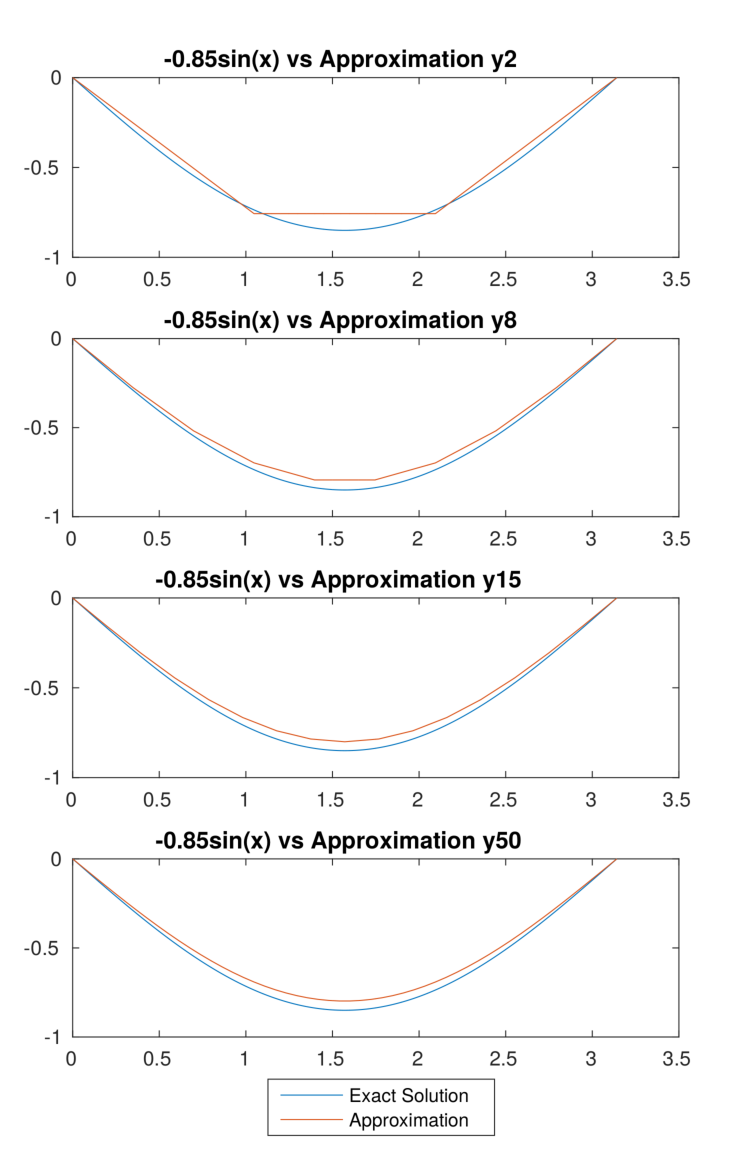
\includegraphics[scale=1.0]{eigenvector_approximation}
    \end{center}
    \caption{Plots of $y=-0.85\sin(x)$ and approximation $y_n$ over the interval $[0, \pi]$
      using the hat basis.}\label{eigen}
  \end{figure}

  We plot the approximations for $n=2, 8, 15, 50$ on the interval $[0, \pi]$
  along with the function $y(x) = -0.85\sin(x)$ in Figure \ref{eigen}. From these
  plots we can see that as we refine the mesh on the interval our approximation
  seems to approach the function $y(x) = C\sin(x)$ for $C = -0.8$ on the interval $[0, \pi]$.
  The function $y(x)=-0.85\sin(x)$ is used as a reference point for the approximation.

\end{proof}
